\chapter[Simulating Fuel Cycles]{Simulating Fuel Cycles}
\section{Simple Verification}

\begin{figure}
	\centering
	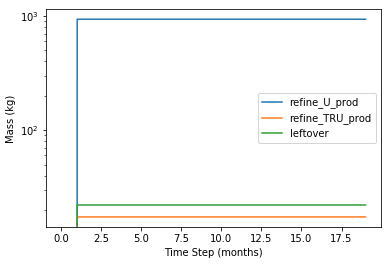
\includegraphics[width=\linewidth]{timeseries-prod}
	\caption{Product time series of a simple simulation.}
	\label{fig:timeseries-prod}
\end{figure}

\begin{figure}
	\centering
	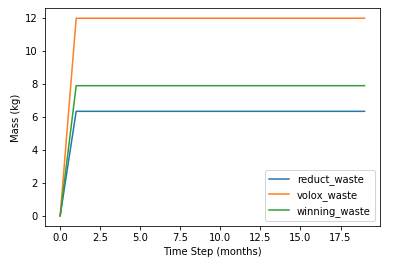
\includegraphics[width=\linewidth]{timeseries-waste}
	\caption{Waste time series of a simple simulation.}
	\label{fig:timeseries-waste}
\end{figure}

\begin{figure}
	\centering
	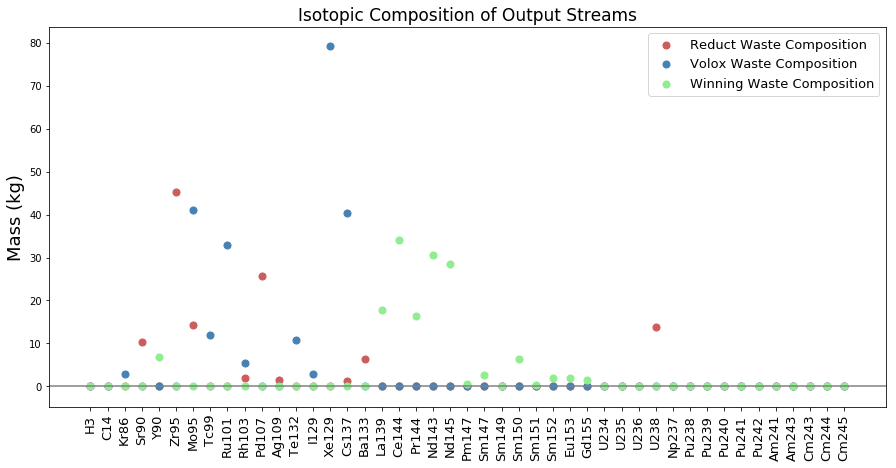
\includegraphics[width=\linewidth]{avg-isotope-comp}
	\caption{Isotopic Composition of Average Waste Streams}
	\label{fig:avg-isotope-comp}
\end{figure}

\begin{figure}
	\centering
	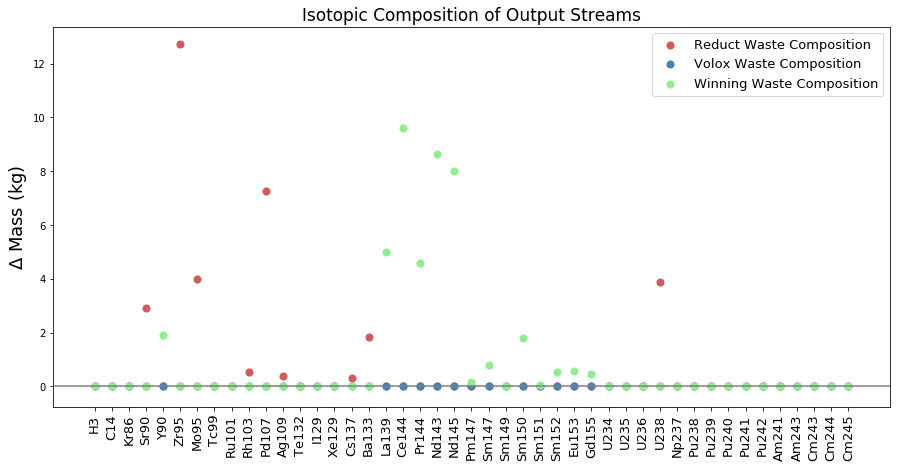
\includegraphics[width=\linewidth]{current-isotope-comp}
	\caption{Isotopic Composition of Current Diverted Waste Streams}
	\label{fig:current-isotope-comp}
\end{figure}

\begin{figure}
	\centering
	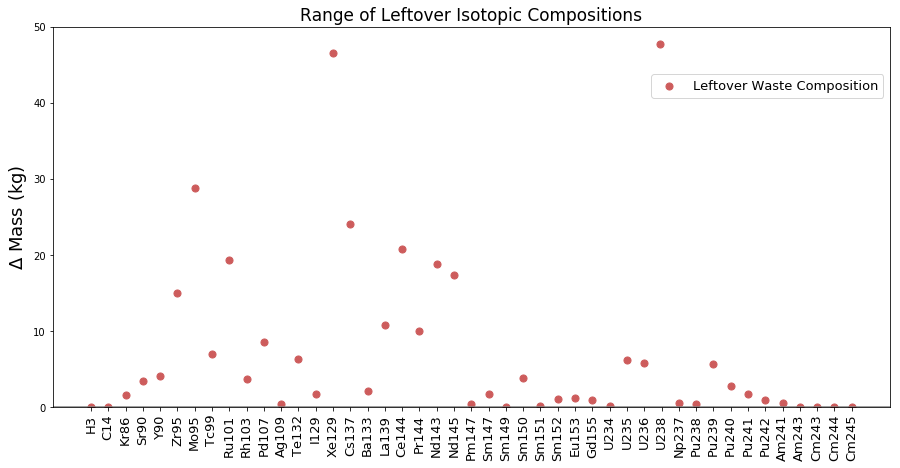
\includegraphics[width=\linewidth]{isotopic-comp-range}
	\caption{Range of Isotopic Values}
	\label{fig:isotopic-range}
\end{figure}

\section{US Fuel Cycle}